\documentclass[10pt]{article}
\usepackage[top=1in, bottom=1in, left=1in, right=1in]{geometry}
\usepackage{float}
\usepackage{color}
\usepackage{picture}
\usepackage{listings}
\usepackage{caption}
\usepackage{hyperref}
\usepackage{graphicx}
\usepackage{amsmath}
\usepackage{subcaption}
\usepackage[utf8]{inputenc}

% Used to change font to Times TX
\usepackage{txfonts}
\usepackage[T1]{fontenc}

% Used for the figures that have been inserted into the document.
\floatstyle{plain} 
\restylefloat{figure}

% Used so as not to indent paragraphs.
\setlength\parindent{0pt}

% Used for syntax highlighting in code.
\definecolor{skyblue}{rgb}{0.53, 0.81, 0.92}
\definecolor{lightred}{rgb}{0.90, 0.36, 0.36}
\definecolor{darkkhaki}{rgb}{0.71, 0.51, 0.06}

% Default parameters for listings package.
\lstset {
	tabsize=4,
	keywordstyle=\color{darkkhaki},
	commentstyle=\color{blue},
	showstringspaces=false,
	stringstyle=\color{lightred},
	frame=TLRB,
	captionpos=b,
	basicstyle=\small\sffamily
}

% Default parameters for hyperref package.
\hypersetup {
	pdftoolbar=true,
	pdfmenubar=true,
	colorlinks=true,
	linkcolor=red,
	citecolor=green,
	filecolor=magenta,
	urlcolor=cyan
}

\begin{document}

\title{\textbf{\textsc{Assignment 5}}}
\author{MA226 : Monte Carlo Simulation \\
			Name: Nikhil Agarwal \\
			Roll No : 11012323 \\
			IIT Guwahati}
\date{}
\maketitle

\begin{center}
	\line(1, 0){15cm}
\end{center}

\section{Problem 1}

\subsection{Statement}

Generate $ 1000 $ standard normal random variables using Double-exponential distribution by acceptance rejection method.
Calculate the constant c, where $\frac{f(x)}{g(x)} <=c $ ,$ f(x) $ and $ g(x) $ are the pdfs of standard Double-exponential distribution respectively.Calculate the theoretical and simulated acceptance probability.How do you justify your generated random numbers are correct? Provide as many verification as you can.

\subsection{Solution}

\subsubsection{Steps followed}
\begin{itemize}
\item First of all we generate the  $ X \sim  (0,1) $ and $ U \sim  (0,1) $ distribution.
\item Secondly we apply inverse transformation method ($ 1 - e^{-{\lambda}v/2} = U  $ for $ y>0 $ and $  e^{-{\lambda}v/2} = U  $ for $ y<0 $)   to convert uniform distribution function to double exponential distribution function.
\item Thus we get $ v= -ln2(1-u) $ for $  u>1/2 $ and $ v= ln(2u)$ for $ u<1/2 $.
\item Then we check for the condition  whether $ x< e^{-{\frac{1}{2}}(v-1)^2} $ for$ u>1/2 $ and  $ x< e^{-{\frac{1}{2}}(v+1)^2}$ for $ u<1/2 $
\item If the condition is true we accept $ Z=V $ else we repeat the process again.
\end{itemize}

\enlargethispage*{1000pt}
\subsubsection{Graph}
\begin{figure}[H]
		\centering
		\resizebox{0.6\linewidth}{!}{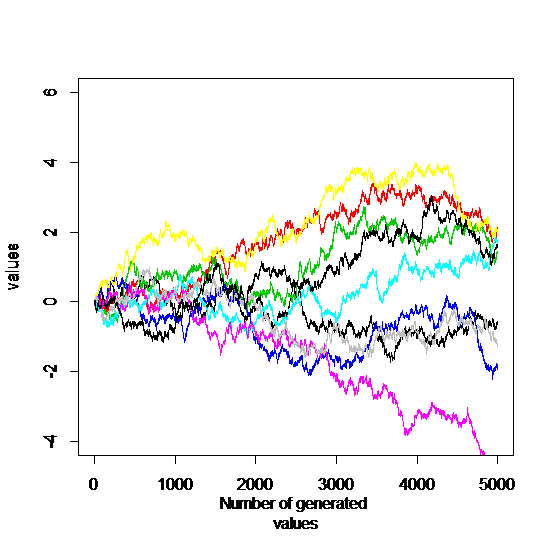
\includegraphics{q1.png}}
		\caption{Normall Distribution in R}
		\label{fig:q1_f1_a}
\end{figure}
\pagebreak



\subsubsection{Results}
\begin{itemize}
\item The value of c  is $\sqrt{\frac{2e}{\pi}} = 1.31548$
\item The Theoretical acceptance probability  is $0.7602$
\item The simulated acceptance probability is $0.75914$
\end{itemize}

\subsubsection{Verification}
The value of mean came out to be $ 0.0147 $ which is quite nearer to 0 and value of variance came out to be $ 1.0118 $ which is quite nearer to 1 . Hence generated numbers are correct.



\subsubsection{R Code}
\lstinputlisting[caption=\texttt{R}  Code which generates the normal variates, label=lst:q1_prog2, language=R]{q1.R}

\pagebreak

\section{Problem 2}

\subsection{Statement}

Do the same exercise for generating random numbers from half-standard normal distribution using exponential distribution with mean 1 by acceptance rejection method.

\subsection{Solution}
\subsubsection{Steps Followed}
\begin{itemize}
\item First of all we generate the  $ X \sim  (0,1) $ and $ U \sim  (0,1) $ distribution.
\item Secondly we apply inverse transformation method ($ 1 - e^{-{\lambda}v/2} = U $ )   to convert uniform distribution function to double exponential  function.
\item Thus we get $ v= -ln(1-u) $ and  $ c= {\sqrt{\frac{e}{2\pi}}}$
\item Then we check for the condition  whether $ v< e^{-{\frac{1}{2}}(v-1)^2} $
\item If the condition is true we accept $ Z=V $ else we repeat the process again.
\end{itemize}
\enlargethispage*{1000pt}
\subsubsection{Graph}
\begin{figure}[H]
		\centering
		\resizebox{0.8\linewidth}{!}{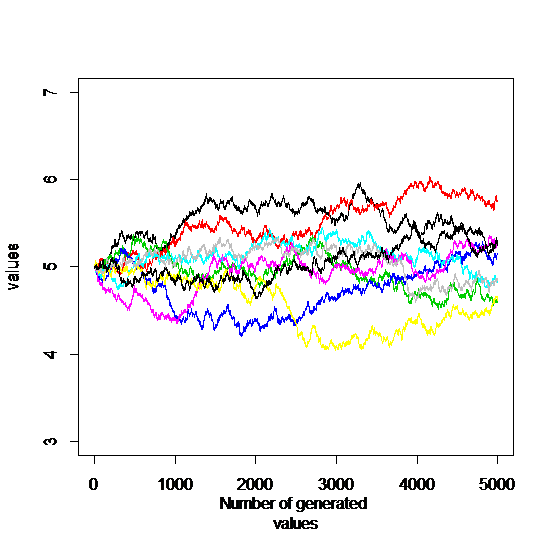
\includegraphics{q2.png}}
		\caption{Normal distribution for $ n=1000 $ in R}
		\label{fig:q2_f1_a}
\end{figure}
\pagebreak


\subsubsection{Results}
\begin{itemize}
\item The value of c  is $\sqrt{\frac{2e}{\pi}} = 1.31548$
\item The Theoretical acceptance probability  is $0.7602$
\item The simulated acceptance probability is $0.759187$
\end{itemize}

\subsubsection{Verification}
The value of mean came out to be $ 0.7957747 $ which is quite nearer to expected mean $ \sqrt{\frac{2}{\pi}} = 0.7979 $ and value of variance came out to be $ 0.3574325 $ which is quite nearer to expected variance $(1-\frac{2}{\pi}) = 0.3634 $ . Hence generated numbers are correct.


\subsubsection{R Code}
\lstinputlisting[caption=\texttt{R} Code which generates the Normal Distribution., label=lst:q2_prog2, language=R]{q2.R}

\pagebreak


\section{Problem 3}

Consider the following discrete distribution.
\begin{center}
\begin{tabular}{cccccc}
j &1 & 2 & 3 & 4 & 5 \\
\hline
j &0.05 & 0.25 & 0.45 & 0.15 & 0.10
\end{tabular}
\end{center}



Qa. Generate 10 random numbers from the above probability mass function using usual procedure(inverse) transform of generating numbers from discrete distribution defined on finite number of points. Calculate mean and variance of generated numbers.\\
Qb.Generate 10 random numbers from the same probability mass function by acceptance rejection principle.Calculate mean and variance of generated numbers.



\subsection{Solution}
\subsubsection{Steps followed}
\begin{itemize}
\item For part a:
\begin {itemize}
\item First of all we generate 10 uniform random numbers.
\item If $P_j <= 0.45 , 0.7 , 0.85 , 0.95 , 1$ output is $ 3 , 2 , 4 , 5 , 1 $ respectively.
\end{itemize}
\item For part b:
\begin {itemize}
\item First of all we generate the  $ X \sim  (0,1) $ and $ U \sim  (0,1) $ distribution.
\item The maximum value of c came out to be 2.25 .
\item Then we have calculated $v=floor(5*u)+1 $ and check for the condition $ v < \frac{f(v)}{4.5}$
\item If the condition is true we accept the output otherwise generate the numbers again.
\end{itemize}
\end{itemize}





\subsubsection{Results}
\begin{itemize}
\item The mean and varince by inverse transformation method is $2.54$ and $1.66667$ respectively.
\item The mean and varince by acceptance rejection principle method is $2.788$ and $2.2345$ respectively.
\end{itemize}

\subsubsection{R Code A}
\lstinputlisting[caption=\texttt{R} Code which generates the  Distribution through inverse transformation method., label=lst:q2_prog2, language=R]{q3.R}
	
\subsubsection{R Code B}
\lstinputlisting[caption=\texttt{R} Code which generates the  Distribution acceptance rejection method., label=lst:q2_prog2, language=R]{q3b.R}

\end{document}
